\documentclass{article}
\usepackage[utf8]{inputenc}
\usepackage{amssymb}
\usepackage{comment}
\usepackage{graphicx}
\usepackage{amsmath,amsfonts,amssymb,amsthm}
\usepackage{mathtools}
\usepackage{commath}

\title{Homework 2}
\author{Vladimir Frants, Yunhua Zhao, Mohamed Ben Zid}
\date{September 2020}

\begin{document}

\maketitle

\section{Exercise 2.6}

\subsection{a)}

From \emph{1.7} the point $\theta^{*}$ we have: 

$$\frac{sin(\alpha_{1}(\theta^{*}))}{sin(\alpha_{2}(\theta^{*}))} = \frac{v_1}{v_2}$$

Multiply both sides by $sin(\alpha_{2}(\theta^{*}))$:

$$sin(\alpha_{1}(\theta^{*}))=\frac{v_{1}\cdot sin(\alpha(\theta^{*}))}{v_{2}}$$

Divide both sides by $v_{1}$:

$$\frac{sin(\alpha_{1}(\theta^{*}))}{v_{1}}=\frac{sin(\alpha_{2}(\theta^{*}))}{v_{2}}$$

$$\frac{sin(\alpha_{1}(\theta^{*}))}{v_{1}} - \frac{sin(\alpha_{2}(\theta^{*}))}{v_{2}} = 0$$

So: 

$$J'(\theta)= \frac{sin(\alpha_{1}(\theta))}{v_{1}} - \frac{sin(\alpha_{2}(\theta))}{v_{2}}$$

Therefore:

$$\theta_{n+1} = \theta_{n} - \epsilon(\frac{sin(\alpha_{1}(\theta_{n}))}{v_{1}} - \frac{sin(\alpha_{2}(\theta_{n}))}{v_{2}})$$

Here we have a vector field: 

$$G(\theta) = \frac{sin(\alpha_{2}(\theta))}{v_{2}} - \frac{sin(\alpha_{1}(\theta))}{v_{1}}$$

A function $G(\theta)$ is Lipschitz-continuous on $\theta\in(-\infty, \infty)$ because it is differentiable at $x\in{(-\infty, \infty)}$ for $v_1 \neq 0, v_2 \neq 0$. 

So we have Lipschitz continuous function $G:\mathbb{R}\rightarrow\mathbb{R}$, and recurison of form:

$$\theta_{n+1}+\epsilon(G(\theta_{n}) + \beta_{\epsilon}(\theta_n)), n\epsilon\leqT$$
with constant step size $\epsilon > 0$ and $\beta_{\epsilon}(\theta_{n})=0$

Let $x_{\epsilon}(t)=\vartheta^{\epsilon}(t), 0\leq t \leq T$, denote the interpolation process of $\{\theta_{n}\}$ on $[0, T]$, for $T > 0$, with $x_{\epsilon}(0)=\theta_{0}$. Because $\sup_{\theta}\lVert\beta_{\epsilon}(\theta)\rVert=0$ the $\epsilon$-indexed sequence of processes ${(x_{\epsilon}(t); 0\leq t \leq T): \epsilon > 0}$ according to the \textbf{theorem 2.3} converges as $\epsilon \rightarrow 0$ (in the sup norm) to the solution of the ODE:

$$ \frac{dx(t)}{dt}=\frac{sin(\alpha_{2}(x(t)))}{v_{2}} - \frac{sin(\alpha_{1}(x(t))}{v_{1}}$$

for $0 \leq t \leq T$.

\subsection{b)}

From the previous section we have have Lipschitz continuous function $G:\mathbb{R}\rightarrow\mathbb{R}$, and recurison of form:

$$\theta_{n+1}+\epsilon(G(\theta_{n}) + \beta_{\epsilon}(\theta_n)), n\epsilon\leqT$$
with constant step size $\epsilon > 0$ and $\beta_{\epsilon}(\theta_{n})=0$

$$G(\theta) = \frac{sin(\alpha_{2}(\theta))}{v_{2}} - \frac{sin(\alpha_{1}(\theta))}{v_{1}}$$

To apply the theorem $2.6$ we need to check the following assumptions:

\begin{enumerate}
    \item $G(\theta)$ is bounded along the trajectory, this is true, because $v1$ and $v2$ are constants and value of $sin(\cdot)$ is in $[-1, 1]$
    \item $\sum_{n}\epsilon_{n}=\infty$, by definition
    \item $\epsilon\rightarrow 0$, by definition
    \item $\sum_{n}\epsilon_{n}\lVert \beta_{n}(\theta_{n})\rVert < \infty$. It is true, because in our case $\beta_{n}(\theta_{n})=0$
\end{enumerate}

Let $x_n(t)=\vartheta(t_{n}+t), t\geq 0$, denote the interpolation process of the shifted sequence $\{\theta_{k}\}$ with $x_{n}(0)=\theta_{n}$. Then as $n\rightarrow\infty$, $x_{n}$ according the theorem \textbf{2.6} converges (in the sup norm) to the solution of the ODE

$$\frac{dx(t)}{dt}=G(x(t))$$. 

Any accumulation point $\theta^{*}$ of $\theta_{n}$ is an asymptotically stable point of $G$, which implies that it is stable and $lim_{t\rightarrow\infty}x(t)=\theta^{*}$.

\subsection{c)}

Here is our simulation for $a=2$, $b=5$, $d=10$, $v_{1}=3$, $v_{2}=1$, and $\epsilon=0.05$. We directly programmed the gradient search method and used $\theta_{0}=10.0$. The method converges to the value $8.283$.

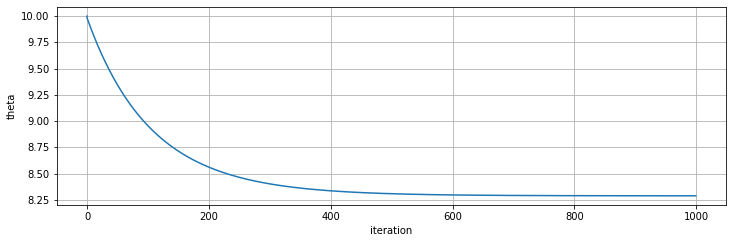
\includegraphics[width=0.9\linewidth]{index.png}



\end{document}
